% Katona's arcs for n=6, k=2. The two arcs that meet {1,2} and avoid each other.
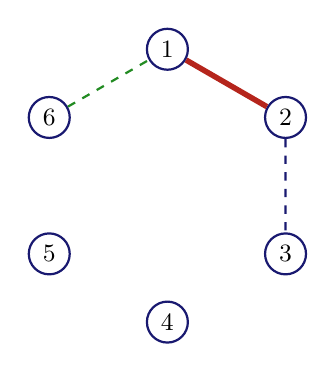
\begin{tikzpicture}[scale=1.05, every node/.style={font=\small}]
  \def\R{1.65}
  \foreach \k in {1,...,6} {
    \pgfmathsetmacro{\ang}{90-(\k-1)*60}
    \node[circle,draw=MidnightBlue,thick,fill=white,inner sep=1.5pt,minimum size=5.2mm]
      (s\k) at (\ang:\R) {$\k$};
  }
  \draw[BrickRed,line width=2pt] (s1) -- (s2);
  \draw[MidnightBlue,thick,dashed] (s2) -- (s3);
  \draw[ForestGreen,thick,dashed] (s6) -- (s1);
\end{tikzpicture}
